\documentclass[]{article}
\usepackage{lmodern}
\usepackage{amssymb,amsmath}
\usepackage{ifxetex,ifluatex}
\usepackage{fixltx2e} % provides \textsubscript
\ifnum 0\ifxetex 1\fi\ifluatex 1\fi=0 % if pdftex
  \usepackage[T1]{fontenc}
  \usepackage[utf8]{inputenc}
\else % if luatex or xelatex
  \ifxetex
    \usepackage{mathspec}
  \else
    \usepackage{fontspec}
  \fi
  \defaultfontfeatures{Ligatures=TeX,Scale=MatchLowercase}
\fi
% use upquote if available, for straight quotes in verbatim environments
\IfFileExists{upquote.sty}{\usepackage{upquote}}{}
% use microtype if available
\IfFileExists{microtype.sty}{%
\usepackage[]{microtype}
\UseMicrotypeSet[protrusion]{basicmath} % disable protrusion for tt fonts
}{}
\PassOptionsToPackage{hyphens}{url} % url is loaded by hyperref
\usepackage[unicode=true]{hyperref}
\hypersetup{
            pdfborder={0 0 0},
            breaklinks=true}
\urlstyle{same}  % don't use monospace font for urls
\usepackage[margin=1in]{geometry}
\usepackage{graphicx,grffile}
\makeatletter
\def\maxwidth{\ifdim\Gin@nat@width>\linewidth\linewidth\else\Gin@nat@width\fi}
\def\maxheight{\ifdim\Gin@nat@height>\textheight\textheight\else\Gin@nat@height\fi}
\makeatother
% Scale images if necessary, so that they will not overflow the page
% margins by default, and it is still possible to overwrite the defaults
% using explicit options in \includegraphics[width, height, ...]{}
\setkeys{Gin}{width=\maxwidth,height=\maxheight,keepaspectratio}
\IfFileExists{parskip.sty}{%
\usepackage{parskip}
}{% else
\setlength{\parindent}{0pt}
\setlength{\parskip}{6pt plus 2pt minus 1pt}
}
\setlength{\emergencystretch}{3em}  % prevent overfull lines
\providecommand{\tightlist}{%
  \setlength{\itemsep}{0pt}\setlength{\parskip}{0pt}}
\setcounter{secnumdepth}{0}
% Redefines (sub)paragraphs to behave more like sections
\ifx\paragraph\undefined\else
\let\oldparagraph\paragraph
\renewcommand{\paragraph}[1]{\oldparagraph{#1}\mbox{}}
\fi
\ifx\subparagraph\undefined\else
\let\oldsubparagraph\subparagraph
\renewcommand{\subparagraph}[1]{\oldsubparagraph{#1}\mbox{}}
\fi

% set default figure placement to htbp
\makeatletter
\def\fps@figure{htbp}
\makeatother


\renewcommand{\href}[2]{#2\footnote{\url{#1}}}
\usepackage{lipsum}
%\usepackage{fancyhdr}
%\pagestyle{fancy}
%\fancypagestyle{plain}

\usepackage[usenames,dvipsnames]{xcolor}
\definecolor{azure(colorwheel)}{rgb}{0.0, 0.5, 1.0}
\definecolor{ultramarineblue}{rgb}{0.25, 0.4, 0.96}

\usepackage{multicol}


\usepackage{pdflscape}



\usepackage[paper=portrait,pagesize]{typearea}
\KOMAoptions{pagesize,  paper=landscape, paper=a4,pagesize,DIV=18,headinclude, footinclude}
\recalctypearea
%\usepackage[margin=1in, landscape]{geometry}
\usepackage[export]{adjustbox}



%\fancyhead{}
%\renewcommand{\headrulewidth}{0pt}

%\fancyhead[R]{
 % \rule[-1.75\baselineskip]{0pt}{0pt}% Strut to ensure a 1/4 \baselineskip between image and header rule
 % \includegraphics[height=3\baselineskip,valign=c]{OECDlogo.jpg}
  %\quad% Space
  % Housing Performance: `r params$ctry_name`
%}

%\fancyfoot[C]{\color{ultramarineblue}OECD Housing Horizontal Project 2021}
%\fancyfoot[RE,RO]{ \thepage}

\usepackage[headsepline]{scrlayer-scrpage}
\pagestyle{scrheadings}



\ifoot{}
\cfoot{ \rule[-1.75\baselineskip]{0pt}{0pt}
  \includegraphics[height=3\baselineskip,valign=c]{OECDlogo.jpg}
  \quad% Space
\scriptsize
\color{ultramarineblue} Housing Horizontal Project 2021}
\ofoot{}

\author{}
\date{\vspace{-2.5em}}

\begin{document}

\chead{
 \rule[-1.75\baselineskip]{0pt}{0pt}
  \includegraphics[height=4\baselineskip,valign=c]{OECDlogo.jpg}
  \quad% Space
   Housing Sector Country Fiche: PRELIMINARY VERSION 15/07/2020}

\newpage

\bigskip

PRELIMINARY VERSION:

prepared by Naomi Cohen, Federica Depace, Maxime Nguyen and Manuel Betin

\begin{itemize}
\item
  This page will be remove for the final version and only two pages will
  remain
\item
  The current version include raw data and raw text as produced by the
  algorithm,
\item
  Fiabilization tests, editorial corrections and validation of data for
  each countries has not been yet undertaken.
\item
  This template is constructed according to data availability and will
  thus display replacement variables if the prefered variables\\
  are not available.
\end{itemize}

\newpage

\color{ultramarineblue} \section{Housing Sector Outcomes: \Large France}

\color{black}

The provision of efficient, sustainable and inclusive housing is crucial
for the well-being of citizens. Housing markets affect people's
well-being through a wide range of channels including access to decent
shelter, environmental quality, efficient use of scarce resources, type
and extent of commuting or its contribution to strong and resilient
economic growth. Galloping urbanisation coupled with increasing
awareness for negative externalities arising from commuting and urban
sprawl have put strain on housing markets and their capacity to deliver
affordable housing to all while reducing environmental and health costs
for current and future generations.

\begin{multicols}{3}

\color{Goldenrod}
\begin{center}
\section{Efficiency}
\end{center}


\begin{center}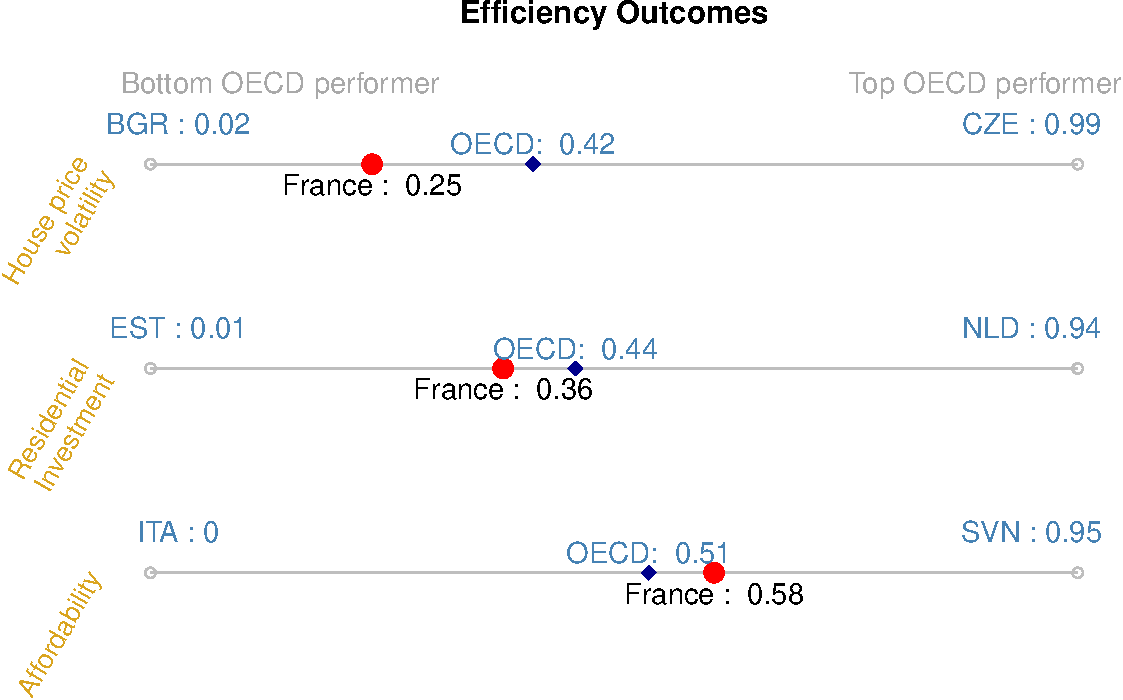
\includegraphics{skeleton_files/figure-latex/Efficiency-1} \end{center}

\color{black}



\footnotesize
Efficiency is defined as the capacity of the sector to provide housing that meets demand across the country, to             facilitate residential mobility and to deliver housing that countributes to macroeconomic stability. The overall performance of France is difficult to assess based on the three main indicators: housing consumption as a share of household expenditure, housing expenditure as a share of disposable income and house price volatility. .The first dimension, housing consumption as a share of household expenditure, is relatively far above OECD average (located in the percentile 0.73). The second one, housing expenditure as a share of disposable income, is slighly above the average (located in the percentile 0.61). Finally, the last selected indicator of efficiency house price volatility, is close to the average (located in the percentile 0.53). Among the factors contributing to those performances we can mention [More from desks]

\columnbreak

\color{ProcessBlue}
\begin{center}
\section{Inclusiveness}
\end{center}

\color{black}


\begin{center}\includegraphics{skeleton_files/figure-latex/Inclusiveness-1} \end{center}





Inclusiveness refers to the capacity of the sector to provide affordable homes across tenure modalities,             to tackle homelessness and to coordinate housing policies across levels of government. The overall performance of France is difficult to assess based on the three main indicators: percent of individuals who changed residence within the last 5 years, share of population able to afford 100 m2 flat with 15 years of income and total overcrowding rate. .The first dimension, percent of individuals who changed residence within the last 5 years, is slightly above OECD average (located in the percentile 0.65). The second one, share of population able to afford 100 m2 flat with 15 years of income, is in the lower third of the distribution (located in the percentile 0.27). Finally, the last selected indicator of inclusiveness total overcrowding rate, is among the 35 percent better performing economies (located in the percentile 0.76). Among the factors contributing to those performances we can mention [More from desks]

\columnbreak

\color{Green}

\begin{center}
\section{Sustainability}
\end{center}

\color{black}


\begin{center}\includegraphics{skeleton_files/figure-latex/Sustainability-1} \end{center}






\end{multicols}

\newpage

\textbackslash{}begin\{tabular\}\{l l\}
\textbackslash{}parbox{[}t{]}\{0.35\textwidth\}\{
\color{ultramarineblue} \section{Housing Sector Policies Variables:}

\small
\color{black} This section is a place holder and do not contain final
variables and text.

\lipsum[2-2]
\bigskip

\begin{center}\includegraphics{skeleton_files/figure-latex/unnamed-chunk-1-1} \end{center}

\end{document}
